\chapter{Modelando la incertidumbre}
\label{sec:algoritmo}
%\section{Agregando probabilidades a un algoritmo existente}
 Las posibles aplicaciones de la generaci\'on de expresiones referenciales que deben referirse al mundo real sufren de \textbf{incertidumbre} por datos ruidosos de sensores y modelos incompletos de la realidad como discutimos en el Cap\'itulo \ref{sec:intro}.
En este cap\'itulo se presentan nuevos algoritmos basados en teor\'ia de modelos y $\+L$-simulaciones como los descriptos en el Cap\'itulo \ref{sec:intro_logica}. Pero que a diferencia de estos usan una distribuci\'on de finita de probabilidades que representa esta incertidumbre. Estos algoritmos generan no \textbf{una} ER, sino un \textbf{ranking} de ERs. Este ranking de expresiones referenciales est\'a ordenado por la probabilidad de ser correctamente interpretada en el contexto. 
Conseguimos as\'i tres caracter\'isticas nuevas de estos algoritmos:
\begin{itemize}
 \item \textbf{No determinismo}: dos ejecuciones del algoritmo con la
misma entrada podr\'{i}an resultar en diferentes ERs para los objetos en la escena. Podemos generar entonces como salida un ranking de las ERs generadas por el algoritmo si lo ejecutamos muchas veces con
el mismo input. 
 \item Conseguimos mayor control sobre la \textbf{sobreespecificaci\'on} que genera el algoritmo, simulando el tipo y la cantidad de sobreespecificaci\'on que encontramos en  corpora.
 \item Dado un corpus de ERs para un dominio determinado,
es posible usar \textbf{aprendizaje autom\'atico} para aproximar una distribuci\'on de probabilidad adecuada para las propiedades y relaciones de una escena no vista antes. Esto hace que el ranking de las ERs generadas para el modelo simule el que se observa en el corpus usado para el aprendizaje autom\'atico.
\end{itemize}
\
Este cap\'itulo est\'a dividido en cinco secciones. En la primer secci\'on explicaremos la entrada y salida del algoritmo. En la Secci\'on \ref{sec:learning} mostraremos como obtener la distribuci\'on de probabilidad finita que toma como entrada el algoritmo, usando aprendizaje autom\'atico cuando hay corpus disponible para el dominio. Luego en la Secci\'on \ref{sec:algoritmo_probabilistico} mostraremos el algoritmo en detalle y definiremos los conceptos y t\'ecnicas de teor\'ia de modelos necesarios para entenderlo. En la Secci\'on \ref{sec:ejemplo_ejecucion} mostraremos un ejemplo de ejecuci\'on paso a paso. Explicaremos c\'omo conseguimos asegurar terminaci\'on, c\'omo se generan las ERs no-determin\'isticamente y c\'omo conseguimos mayor control sobre la sobreespecificaci\'on. Finalmente en la Secci\'on \ref{sec:link-algoritmo} daremos un resumen y comentaremos c\'omo se linkea el cap\'itulo con el resto de la tesis.

\section{Entrada y salida del algoritmo probabil\'istico}
\label{input_algo}
Como todo algoritmo de GER, nuestros algoritmos toman como entrada un contexto representado por un \textbf{modelo} $\+M$. Por ejemplo en la Figura \ref{figura-y-modelo} se muestra el modelo de la escena de la izquierda. Sin embargo a diferencia de otros algoritmos, nuestros algoritmos no toman como entrada el \textbf{target}. Nuestros algoritmos generan rankings de ERs para todos los elementos del modelo paralelamente. En particular, el algoriitmo generar\'a ERs para el conjunto singleton \{$e_5$\}. En la Secci\'on \ref{sec:genera_plural} de este cap\'itulo se muestra una sencilla extensi\'on de los algoritmos que permite generar ERs plurales.
\begin{figure}[h]
\begin{subfigure}{.5\textwidth}
  \centering
	%\vspace*{-.2cm}
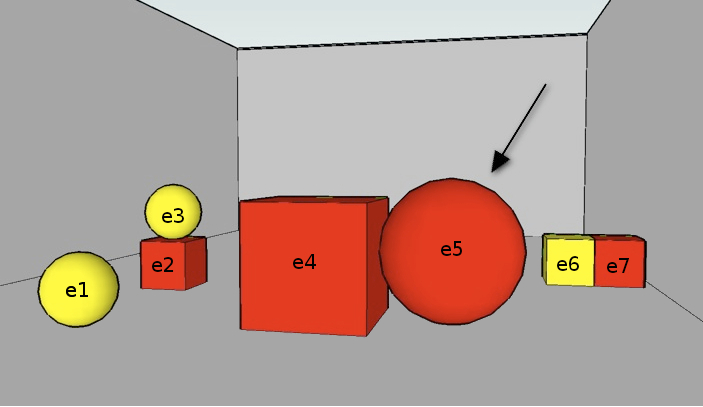
\includegraphics[width=\textwidth]{images/22.jpg}
 % \caption{}\label{GRE3D7-stimulus1-ids-modelo-y-figura}
\end{subfigure}
\begin{subfigure}{.5\textwidth}
  \centering
%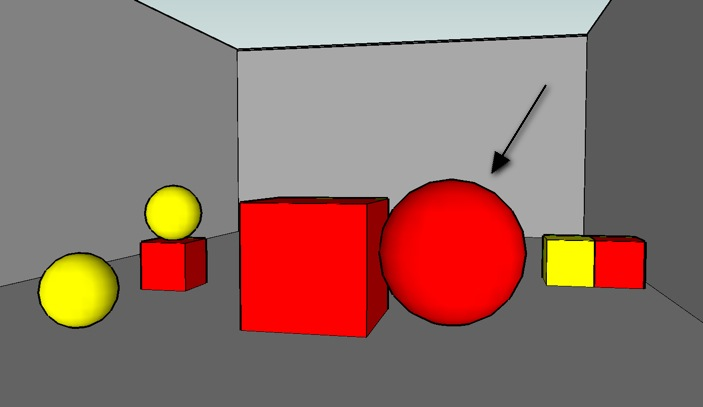
\includegraphics[width=\textwidth]{images/22sinletras.jpg}
%%\caption{Ejemplo de contexto}
%\label{GRE3D7-stimulus1-b}
\vspace*{1cm}
\begin{picture}(250,0)
\put(0,-50){\begin{tikzpicture}
  [
    n/.style={circle,draw,inner sep=1.5pt,node distance=1.5cm},
		 aArrow/.style={->, >=stealth, semithick, shorten <= 1pt, shorten >= 1pt},
  ]
 \node[n,label=below:{
    \relsize{-2}$\begin{array}{c}
      \nSmall\\[-3pt] 
      \nYellow \\[-3pt] 
      \nBall\end{array}$}] (a) {$e_1$};
 \node[n,label=below:{
    \relsize{-2}$\begin{array}{c}     
      \nSmall\\[-3pt] 
      \nRed\\[-3pt] 
      \nCube\end{array}$}, right of=a] (b) {$e_2$};
 \node[n,label=above:{
    \relsize{-2}$\begin{array}{c}     
      \nSmall\\[-3pt] 
      \nYellow\\[-3pt] 
      \nBall\end{array}$}, above of=b] (c) {$e_3$};
 \node[n,label=below:{
    \relsize{-2}$\begin{array}{c}
      \nLarge\\[-3pt] 
      \nRed\\[-3pt] 
      \nCube\end{array}$}, right of=b] (d) {$e_4$};
 \node[n,label=below:{
    \relsize{-2}$\begin{array}{c}
      \nLarge\\[-3pt] 
      \nRed\\[-3pt] 
      \nBall\end{array}$}, right of=d] (e) {$e_5$};
 \node[n,label=below:{
    \relsize{-2}$\begin{array}{c}
      \nSmall\\[-3pt] 
      \nYellow\\[-3pt] 
      \nCube\end{array}$}, right of=e] (f) {$e_6$};
 \node[n,label=below:{
    \relsize{-2}$\begin{array}{c}
      \nSmall\\[-3pt]
      \nRed\\[-3pt] 
      \nCube\end{array}$},  right of=f] (g) {$e_7$};
 \draw [aArrow,bend right=40] (b) to node[auto,swap]{\relsize{-3}$\nBelow$} (c);
 \draw [aArrow,bend right=40] (c) to node[auto,swap]{\relsize{-3}$\texttt{ontop}$} (b);
 \draw [aArrow,bend right=40] (d) to node[auto,swap]{\relsize{-3}$\nLeftof$} (e);
 \draw [aArrow,bend right=40] (e) to node[auto,swap]{\relsize{-3}$\nRightof$} (d);
 \draw [aArrow,bend right=40] (f) to node[auto,swap]{\relsize{-3}$\nLeftof$} (g);
 \draw [aArrow,bend right=40] (g) to node[auto,swap]{\relsize{-3}$\nRightof$} (f);
 %\draw[dotted] (-0.5,-1.3) rectangle (8,3.1);
 \draw[dotted] (-0.5,-1.5) rectangle (8,3);
 \end{tikzpicture}}
 \end{picture}
 %\end{flushleft}

%\vspace*{2cm} 
 %\caption{}\label{representacion-modelo-y-figura}

\end{subfigure}%
\caption{Modelo que representa a la figura.}
\label{figura-y-modelo}
\end{figure}


El sistema tambi\'en toma como entrada una \textbf{distribuci\'on de probabilidad finita} de las propiedades y relaciones de la signatura del modelo\footnote{En lo que sigue nos referiremos a las propiedades y relaciones de un modelo simplemente como relaciones, distinguiendo entre relaciones unarias (propiedades) o relaciones binarias (relaciones) cuando sea necesario.}. Una distribuci\'on de probabilidades Rs, es una lista de pares (R, R.\puse) que vinculan a cada relaci\'on R a una cierta probabilidad de uso R.\puse\ ordenada de mayor a menor por \puse. La distribuci\'on de probabilidad para el modelo del ejemplo se ilustra en la Tabla \ref{probabilidades-escena}.  

\begin{table}[h]
\begin{center}
\footnotesize{
\begin{tabular} {  l c c c c c c c c c c}
\hline
%\multicolumn{1}{c}{}
%&\multicolumn{1}{c}{Domain}
%&\multicolumn{3}{c}{Descriptions}\\

R				&{\it ball}			& {\it cube}	& {\it red}	  & {\it large} & {\it ontop} & {\it yellow} & {\it small} & {\it rightof} & {\it leftof} & {\it below}   \\
\hline
R.\puse	& 1.0			& 1.0		& 0.978	& 0.257 & 0.178 & 0.15   & 0.107 & 0.007& 0 &0\\
\hline

\end{tabular}
}
\end{center}
\vspace*{-.5cm} 
\caption{Distribuci\'on de probabilidad de las propiedades y relaciones de la Figura \ref{figura-y-modelo}.}\label{probabilidades-escena}

\end{table}
%esfera 1.0, \\
%cube 1.0,\\
%rojo 0.978,\\ 
%large 0.257,\\ 
%ontop 0.178,\\ 
%yellow 0.15,\\
%peque\~no 0.107,\\ 
%izquierda 0.007,\\
%arriba 0.007, \\
%derecha 0, \\
%leftof 0, \\
%a-la-der-de 0, \\
%belowof 0\\

Sea $\REL$ es el
conjunto de todos los s\'imbolos de relaci\'on en el modelo (es decir, la~\emph{signatura} del modelo), entonces podemos decir que Rs $\in (\REL \times [0,1])^*$. En la pr\'oxima secci\'on explicaremos como obtener estas probabilidades que el algoritmo toma como input.
Los algoritmos descriptos en el Cap\'itulo \ref{sec:seleccion} y en el Cap\'itulo \ref{sec:intro_logica} procesan las relaciones unarias y las relaciones binarias de forma diferente. Adem\'as, en general prefieren usar primero las relaciones unarias y s\'olo recurrir a las binarias en caso de que sea necesario. Como se ha observado previamente en trabajo emp\'irico~\cite{viet:gene11}, hay escenas en las cuales las personas usan relaciones binarias antes que unarias y aunque no sea necesario usarlas. Por lo tanto para uniformizar el tratamiento de todas las relaciones sin importar su aridad nuestro algoritmo modifica el modelo $\gM$ antes de comenzar transformando todas las relaciones a binarias. Esto se hace agregando un elemento extra \emph{dummy} al modelo que no representa ning\'un objeto de la escena y que se relaciona con todos los objetos que ten\'ian relaciones unarias. Por ejemplo, en la Figura \ref{figura-y-modelo} se codifica el hecho de que $e_1$ es amarillo diciendo que est\'a relacionado con el elemento \emph{dummy} por la relaci\'on binaria \emph{yellow}. 

Como explicamos en el Cap\'itulo \ref{sec:intro_logica}, la salida el algoritmo es lo que se llaman las $\mathcal {L}$-clases (clases de la l\'ogica $\mathcal {L}$) de semejanza del modelo de entrada $\gM $. Intuitivamente, si dos elementos en el modelo pertenecen a la misma $\mathcal {L}$-clase de semejanza, entonces el lenguaje~$\mathcal {L}$ no es lo suficientemente expresivo para diferenciarlos (es decir, no hay una f\'ormula en~$\mathcal {L }$ que pueda distinguirlos). Cada  $\mathcal {L}$-clase va acompa\~nada de un conjunto de f\'ormulas cuyas interpretaciones en el modelo de input coinciden con la $\mathcal {L}$-clase. Estas f\'ormulas son las expresiones referenciales que referencian a los elementos de la $\mathcal {L}$-clase. Si las $\mathcal {L}$-clases son conjuntos singleton, el algoritmo lleg\'o a un punto fijo y termina. En otra etapa de postprocesamiento se identifica la f\'ormula cuya extensi\'on es igual al target como una ER del target. Como el algoritmo es no determin\'istico el ranking que ERs de la salida se genera ejecutando el algoritmo un n\'umero n de veces. Cada ER generada tiene asociada una probabilidad calculada como una combinaci\'on de los \puse\ de las relaciones que contiene la ER. El ranking de ERs se genera ordenando las ERs de acuerdo a la frecuencia con la cual el algoritmo la genera, la cual se correlaciona con la probabilidad antes mencionada.

%La salida del algoritmo es un conjunto de f\'ormulas y sus interpretaciones en el modelo (que ser\'a ER de un target singleton, si la interpretaci\'on de la f\'ormula contiene s\'olo 1 objeto) de los elementos del modelo. Si al terminar el algoritmo la interpretaci\'on de cada f\'ormula tiene un s\'olo elemento, tenemos una ER que identifica al elemento, para cada elemento del modelo. 

\section{Probabilidades de uso}
\label{sec:learning}

En la secci\'on anterior dijimos que el algoritmo asume que para cada relaci\'on R del modelo se tiene una probabilidad de uso R.\puse. Como dijimos, nuestro algoritmo es no-determinista: en 2 ejecuciones podr\'ia dar ERs diferentes para el mismo target y la misma lista de probabilidades de uso. Las probabilidades de uso son el motor que gu\'ia este no-determinismo. Como explicaremos en la Secci\'on \ref{sec:algoritmo_probabilistico}. En esta secci\'on describimos c\'omo obtener la distribuci\'on finita de probabilidades de las relaciones de la signatura del modelo de entrada. Primero explicamos c\'omo calcularlas en el caso de tener corpus disponible para la escena. Luego generalizamos nuestro enfoque al caso de tener que generar ERs para una escena no vista antes usando t\'ecnicas de aprendizaje autom\'atico.  

%\begin{figure}[h]
%\centering
%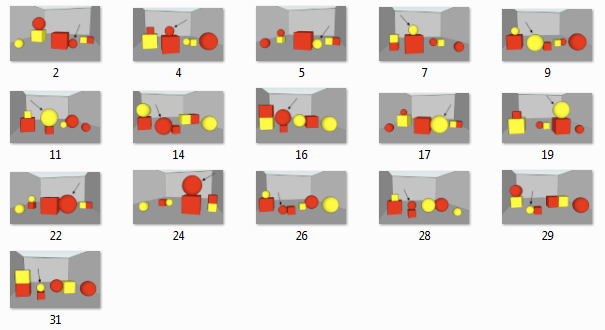
\includegraphics[width=1\textwidth]{images/rojo-amarillo.png}
%\caption{Im\'agenes del \textit{GRE3D7} parte rojo y amarillo}
%\label{rojo-amarillo}
%\end{figure}

\subsection{Calculando \puse\ cuando hay disponible un corpus para la escena}
\label{sec:learning-corpus}

Supongamos que queremos generar autom\'aticamente una ER para el target $t$ en una
determinada escena, y que tenemos disponible un corpus $C$ de ERs de $t$
en esa escena.

%En la Figura \ref{verde-azul} se muestran las escenas mostradas a los participantes del corpus \textit{GRE3D7} introducido en la Secci\'on \ref{sec:corpusGRE}, esta parte incluye s\'olo las escenas verde y azules. El corpus contiene otra parte similar con colores rojo y amarillo.


%El corpus tiene para cada imagen 140 ERs dadas por personas. La Figura \ref{fig4-4} muestra una escena y las distintas ERs que aparecieron en el corpus.
%Las ERs dadas en Figura \ref{fig4-4} son las ERs diferentes que est\'an en el corpus para el contexto mostrado en la misma figura. Viendo esas ERs, uno podr\'ia imaginarse que no son las del corpus mismo, ya que diferentes personas normalmente usan distintas palabras para nombrar al mismo objeto, distintas frases, distinto orden de las palabras, s\'i es verdad, este corpus ya ha sido procesado para filtrar todas esas cosas, dejando un vocabulario com\'un a todas las ERs, si bien es verdad que con eso perdemos informaci\'on por ejemplo de la realizaci\'on particular que hizo una persona, pero ganamos en poder agrupar las ERs por la informaci\'on que la persona incluy\'o, en la etapa de selecci\'on de contenido de la ER. Si quisi\'eramos partir de un corpus con las ERs tal cual dieron las personas, tendr\'iamos que realizar los siguientes pasos a fin de unificar el vocabulario:

Antes de dar la metodolog\'ia para calcular las probabilidades de uso, explicaremos qu\'e hacer con un corpus de ERs para tener unificado el vocabulario, y poder as\'i definir el conjunto de relaciones a usar en las ERs. A continuaci\'on describimos los pasos:

\begin{enumerate}
\item \textbf{Tokenizar} las expresiones referenciales y llamar al conjunto de palabras distintas
 $Pal$. %En particular, las expresiones de varias palabras como {\it arriba de}, {\it encima de}
  %deben ser igualadas a una \'unica palabra que signifique lo mismo, digamos \emph{ontop}.

\item \textbf{Eliminar hiper\'onimos} de $Pal$. Por ejemplo, si ambos \emph{cubo} y
  \emph{cosa} aparecen en $Pal$ para nombrar lo mismo, eliminar \emph{cosa}, ya que \emph{cubo} es m\'as espec\'ifico.

\item \textbf{Normalizar sin\'onimos} si el conjunto de palabras obtenidas en los pasos anteriores contiene
  sin\'onimos hay que normalizarlos con un representante de la clase. Por ejemplo, las palabras \emph{chico}
  y \emph{peque\~no} son ambas representadas por la sem\'antica \emph{small}.

\item \textbf{Llamar $\REL$} al conjunto resultante, de la etapa anterior; que ser\'a la signatura del modelo $\gM$ que utilizar\'a el algoritmo.

\item \textbf{Definir $\gM$} para cada escena, tal que la interpretaci\'on
 $\interp {\cdot}$ asegure de que todas las ERs encontradas en el corpus sean ERs en
  el modelo. Por ejemplo, las ERs de la Figura \ref{fig4-4} deben denotar el target se\~nalado en la figura, siendo el modelo 
$\gM$ considerado el representado en Figura~\ref{fig4-4}.
%GRE3D7-stimulus-cap2
\item \textbf{Calcular R.\puse\ }para cada R$\in \REL$ utilizando la siguiente f\'ormula: Si
  hay muchas ERs para cada escena (como es el caso del corpus \textit{GRE3D7}) $R.\puse\ = \#ERs$ que tienen R $/\#ERs$ en el corpus o asignamos 1 a R.\puse \ si R est\'a en la ER, asignamos 0 en caso contrario (como es el caso del corpus TUNA).
\end{enumerate}

\begin{figure}[h]
\begin{subfigure}{.4\textwidth}
\centering
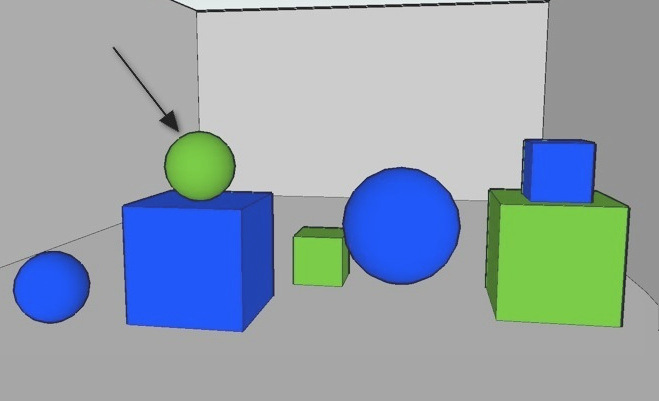
\includegraphics[width=\textwidth]{images/3.jpg}
%\vspace*{1cm}
%\caption{Contexto 3 del GRE3D7}
\end{subfigure}
%\hspace*{1cm}
\begin{subfigure}{.58\textwidth}

%\begin{figure}[h]
\centering
\begin{tikzpicture}
  [
    n/.style={circle,draw,inner sep=3pt,node distance=2cm},
    aArrow/.style={->, >=stealth, semithick, shorten <= 1pt, shorten >= 1pt},
  ]
 \node[n,label=below:{
    \relsize{-1}$\begin{array}{c}
      \nLeft\\[-2pt]
      \nSmall\\[-2pt] 
      \nBlue\\[-2pt]
      \nBall\end{array}$}] (a) {$e_1$};

 \node[n,label=below:{
    \relsize{-1}$\begin{array}{c}
      \nLeft\\[-2pt]
      \nBig\\[-2pt] 
      \nBlue\\[-2pt]
      \nCube\end{array}$}, right of=a] (b) {$e_2$};

 \node[n,label=above:{
    \relsize{-1}$\begin{array}{c}
      \nTop\\[-2pt]      
			\nLeft\\[-2pt]
      \nSmall\\[-2pt]      
			\nGreen\\[-2pt]
      \nBall\end{array}$}, above of=b] (c) {$e_3$};

 \node[n,label=below:{
    \relsize{-1}$\begin{array}{c}
      \nSmall\\[-2pt] 
      \nGreen\\[-2pt] 
      \nCube\end{array}$}, right of=b] (d) {$e_4$};

 \node[n,label=below:{
    \relsize{-1}$\begin{array}{c}
      \nBig\\[-2pt] 
      \nBlue\\[-2pt] 
      \nBall\end{array}$}, right of=d] (e) {$e_5$};

 \node[n,label=below:{
    \relsize{-1}$\begin{array}{c}
      \nBig\\[-2pt] 
      \nGreen\\[-2pt] 
      \nCube\end{array}$}, right of=e] (f) {$e_6$};

 \node[n,label=above:{
    \relsize{-1}$\begin{array}{c}
      \nTop\\[-2pt]
      \nSmall\\[-2pt]
      \nBlue\\[-2pt]
      \nCube\end{array}$}, above of=f] (g) {$e_7$};

 \draw [aArrow,bend right=90] (b) to node[auto,swap]{\relsize{-1}$\nBelow$} (c);
 \draw [aArrow,bend right=90] (c) to node[auto,swap]{\relsize{-1}$\texttt{ontop}$} (b);

 \draw [aArrow,bend right=30] (d) to node[auto,swap]{\relsize{-1}$\nLeftof$} (e);
 \draw [aArrow,bend right=30] (e) to node[auto,swap]{\relsize{-1}$\nRightof$} (d);

 \draw [aArrow,bend right=90] (f) to node[auto,swap]{\relsize{-1}$\nBelow$} (g);
 \draw [aArrow,bend right=90] (g) to node[auto,swap]{\relsize{-1}$\texttt{ontop}$} (f);
\draw[dotted] (-0.5,-2.4) rectangle (10,4.7);
 %\draw[dotted] (-.65,-1.2) rectangle (7.1,2.1);

 \end{tikzpicture}
%\vspace*{-.4cm}\caption{Representaci\'on de las propiedades y relaciones, como un grafo etiquetado, del contexto de la Figura \ref{fig4-4}.}
\label{fig4-5}
%\end{figure}

\end{subfigure}
\caption{Contexto y modelo.}\label{fig4-4}
\end{figure}

En el caso del corpus \textit{GRE3D7} el vocabulario unificado es 
$\REL = \{ball, cube, large, small,\\
green, red, yellow, blue, right, left, top, center, rightof, leftof, ontop,
below\} $.

 Utilizamos las ERs del corpus $C$
para definir el modelo relacional utilizado por el algoritmo. Entonces 
definimos el valor de \puse\ para cada una de las relaciones en el modelo como el
porcentaje en que aparece la relaci\'on en las ERs. Es decir,
\begin{equation} \label{eq1}
R.\puse = \frac {\#\mbox{de ERs en $C$ en el que aparece R}} {\#\mbox{de las ERs en $C$}}.
\end{equation}

Por ejemplo {\it ball} del ejemplo de la Figura \ref{fig4-4}, aparece en todas las ERs del corpus es decir 140, entonces {\it ball}.\puse=1 ya que 140/140=1, en cambio {\it green} aparece en 137 ERs, entonces {\it green}.\puse=0.98 ya que 137/140=0.98.

Esta estimaci\'on es simplista y, por ejemplo, no 
diferencia las propiedades del target y las propiedades de
los landmarks utilizadas en una ER relacional para completar la descripci\'on
del target. Pero es intuitiva y no requiere parsear las ERs para distinguir entre target y landmark. Como vamos a ver
en el Cap\'itulo~\ref{sec:evaluacion} produce ERs naturales
que coinciden con las encontradas en corpora.

Veamos ahora el siguiente ejemplo, el contexto y el modelo se muestra en la Figura \ref{fig4-4}.


Las ERs, cantidad de ocurrencias y porcentaje del corpus para de la Figura~\ref{fig4-4} se muestran en la Tabla~\ref{corpus-distribution}. La signatura resultante y su \puse\ asociado se muestran en la Tabla~\ref{probability-of-use}.\\

El \puse de las relaciones taxon\'omicas fue reemplazado por 1 ignorando el \puse conseguido por el m\'etodo para evitar que el algoritmo genere ERs como {\it la esfera que est\'a sobre algo}.

\begin{table}[h!]
\begin{center}
\begin{tabular}{|l|c|c|}
\hline
Expresiones Referenciales & Cantidad de ocurrencias & Porcentaje \\
\hline

green ball & 91 & 65.00\% \\
small green ball   & 23 & 16.43\% \\
small green ball on-top red large cube & 8 & 5.71\% \\
green ball on-top blue cube & 5 & 3.57\% \\
green ball on-top large blue cube & 5 & 3.57\% \\
small green ball on-top blue cube & 2 & 1.43\% \\
ball on-top cube & 1 & 0.71\% \\
small green ball on-top red large left cube  & 1 & 0.71\% \\
small ball on-top large cube & 1 & 0.71\% \\
top green ball  & 1 & 0.71\% \\
small ball on-top cube & 1 & 0.71\% \\
green ball on-top cube & 1 & 0.71\% \\

\hline
\end{tabular}
\caption{Sem\'antica de las expresiones referenciales producidas por las personas para la Figura~\ref{fig4-4}.}\label{corpus-distribution}
\end{center}
\end{table}

Observe que los valores R.\puse\ obtenidos de esta manera deben ser
interpretados como la probabilidad de utilizar R para describir el target en
modelo de $\gM $, y podr\'{i}amos argumentar que se correlacionan con la
 saliencia de R para el target y su modelo. 
 
Estas probabilidades no ser\'an \'utiles
para describir los diferentes targets en diferentes escenas poruqe son dependientes de la escena para la que se calcularon. Veremos c\'omo se
pueden obtener valores para otros targets y escenas utilizando un
enfoque de aprendizaje autom\'atico en la siguiente secci\'on. 


\begin{table}[H]
\begin{center}
\begin{tabular}{ccccccccccccc}
\hline
\it{ball} & \it{cube} &  \it{green} & \it{small} &  \it{ontop} &  \it{blue} &  \it{large} &  \it{left} &  \it{top} &\it{right} &  \it{leftof} &    \it{rightof} &\it{below} \\
\hline

1.0 & 1.0 & 0.978 &0.257 &0.178 & 0.125 &0.107  &0.007  &0.007 & 0 &0&0&0\\
\hline
\end{tabular}
\caption{Probabilidades de uso de las palabras del corpus \textit{GRE3D7} obtenidas usando la F\'ormula \ref{eq1} para la Figura \ref{fig4-4}.}  
\label{probability-of-use}
\end{center}
\end{table}



\subsection{Calculando \puse\ para el target para escenas sin corpus } 
\label{subsec:learning}

%If there is no corpora that describes the target we can estimate the
%\puse~from corpora on a different scenes in the same domain.
%
%We use simple features to obtain the function, all the features can be
%extracted automatically from the relational model and are listed in


Si no hay corpus de expresiones referenciales para la escena, se puede estimar las \puse~a partir de corpus de
diferentes escenas en el mismo dominio.

En lo que sigue introduciremos regresi\'on lineal que es la t\'ecnica de aprendizaje autom\'atico que usaremos para estimar las probabilidades de uso \puse\ de las palabras que le daremos al algoritmo, y luego daremos un ejemplo de c\'omo calculamos las probabilidades de uso para una figura particular del \textit{GRE3D7}. La \textbf{regresi\'on lineal} es un modelo matem\'atico usado para aproximar la relaci\'on de dependencia entre una variable dependiente Y, las variables independientes $X_i$ y un t\'ermino aleatorio $\varepsilon$. Este modelo puede ser expresado como:

    $Y_t = \beta_0 + \beta_1 X_1 + \beta_2 X_2 + \cdots +\beta_p X_p + \varepsilon$ donde:
\begin{itemize}
    \item $Y_t$: variable dependiente, explicada o regresando.
    \item $X_1$, $X_2$, $\cdots$, $X_p$ : variables explicativas, independientes o regresores.
    \item $\beta_0$,$\beta_1$,$\beta_2$,$\cdots$,$\beta_p$ : par\'ametros, miden la influencia que las variables explicativas tienen sobre Y. Donde $\beta_0$ es la intersecci\'on o t\'ermino {\it constante}, las $\beta_i$ \ (i > 0) son los par\'ametros respectivos a cada variable independiente, y $p$ es el n\'umero de par\'ametros independientes a tener en cuenta en la regresi\'on.
\end{itemize}
Tomaremos la parte azul y verde del corpus \textit{GRE3D7} mostrado en la Figura \ref{verde-azul} del Ap\'endice \ref{imagenesGRE3D7-apendice}, para aprender las probabilidades de uso de cada palabra de las ERs que dieron las personas, y as\'i estimar c\'omo es la distribuci\'on de las probabilidades de uso de las palabras del conjunto $REL$ en el corpus.

Para la tarea de aprendizaje autom\'atico definimos un conjunto de caracter\'isticas de las ERs. Estas caracter\'isticas son las variables $X_i$ que le daremos al m\'etodo de regresi\'on lineal para calcular la dependencia o independencia de la probabilidad de uso \puse\ de cada palabra con respecto a ellas.

Las caracter\'isticas que seleccionamos son:

\begin{itemize}
\item target-tiene 1 cuando el elemento target tiene la propiedad. 
\item \#rel-prop  n\'umero de propiedades y relaciones que el target tiene.
\item \#rel  n\'umero de relaciones binarias que el target tiene. 
\item landmark-tiene 1 cuando un landmark del target tiene la propiedad. Un objeto es un landmark si tiene una relaci\'on directa en el modelo, con el target.
\item location-has 1 cuando la ER puede usar la ubicaci\'on del target en la figura\footnote{Esto se hizo porque el TUNA corpus tiene algunas ERs donde se le dijo a la gente que pod\'ian usar la localizaci\'on del objeto y otras que no.}.
\item disc 1 sobre el n\'umero de objetos en el modelo que tienen la propiedad.  
adj-target-tiene n\'umero de adjetivos que la ER contiene.
\end{itemize}

El procedimiento entonces fue el siguiente:
Creamos un archivo por cada palabra del vocabulario $\REL$. En cada l\'inea del archivo 
se escribieron la lista de propiedades nombradas anteriormente, por cada ER de la imagen considerada. Cada archivo fue analizado con la funci\'on de regresi\'on lineal de WEKA \cite{Hall:WEK09}, que tiene una colecci\'on de herramientas para aprendizaje autom\'atico.

En la Tabla \ref{tabla-linear-regresion-all} se muestra la salida del algoritmo de regresi\'on lineal para las 16 escenas verde y azules del corpus GRE3D7 y sus respectivas ERs. En la primer columna podemos ver la palabra, 
en la segunda columna est\'a el error promedio dado por regresi\'on lineal, en la tercera columna el error medio 
y en la cuarta la f\'ormula que la regresi\'on lineal calcul\'o para la probabilidad de uso de la palabra considerada.

\begin{table}[h]
\begin{center}
\begin{tabular}{|l|c|c|l|}
\hline
Palabra &Error promedio	LR	& Error-PM	& F\'ormula de LR\\
\hline
ball		 &0.0465   &0.0609	  & 0.2894 * disc + 0.7883\\
\hline
cube		 &0.0417	 &0.0531	  &0.49   * disc - 0.0129\\
\hline
\hline
blue		 &0.0353	 &0.0454	  &0.848  * target-tiene + 0.1073\\
\hline
green		 &0.0264	 &0.046	    &0.8722 * target-tiene + 0.0016\\
\hline
\hline
large		 &0.1762	 &0.2378	  &0.5911 * target-tiene + 0.0354\\
\hline
small		 &0.1499	 &0.1755	  &0.3918 * target-tiene + 0.2478 * landmark-tiene -\\
				 &				 &					&0.0913\\
\hline
\hline
leftof  &0.0041	 &0.0094	  &0.0131 * target-tiene +\\
				 &				 &					&0.0253 * adj-target-tiene - 0.0507\\
\hline
ontop	 &0.0706	 &0.1594	  &0.2942 * target-tiene \\
\hline
rightof &0.0029	 &0.0049	  &0.0153 * target-tiene + 0.001\\
\hline
\hline
left		 &0.0068	 &0.0101	  &0.0346 * adj-target-tiene - 0.0653\\
\hline
right		 &0.0079	 &0.0092	  &-0.0118 * disc + 0.0141\\
\hline
top    &0.0099 	 &0.0135		& 0.0069\\
\hline
center	 &0.0023	 &0.0037	  &0.0047 * target-tiene + 0.0047 * adj-target-tiene +\\
				 &				 &					&0.0029 * landmark-tiene - 0.009\\
\hline
\end{tabular}
\caption{F\'ormulas y errores de regresi\'on lineal para la parte del corpus \textit{GRE3D7} que se muestra en la Figura \ref{verde-azul} del Ap\'endice \ref{imagenesGRE3D7-apendice}.}
\label{tabla-linear-regresion-all}
\end{center}
\end{table}

Las palabras {\it red} y {\it yellow} no aparecen en la Tabla \ref{tabla-linear-regresion-all} porque no aparec\'ian en las ERs del corpus de las im\'agenes consideradas (las que conten\'ian colores verdes y azules).

%\textbf{A ESTA TABLA LE FALTAN 3... DEBERIA AGREGARLAS!}

%En la Tabla \ref{tabla-linear-regresion-all} se muestran 4 columnas: en la primer columna podemos ver la palabra, 
%en la segunda columna est\'a el error promedio dado por regresi\'on lineal, en la tercera columna el error medio 
%y en la cuarta la f\'ormula que regresi\'on lineal calcul\'o para la probabilidad de uso de la palabra considerada. 

Podemos ver por ejemplo que {\it ball} tiene una \puse\ alta, es natural ya que en el corpus GRE3D7 todos los targets son {\it ball}. En cambio se puede ver que en {\it cube} no es tan alto y la \puse depende m\'as de la discernibilidad (disc). La \puse\ de {\it cube} representa en este dominio la probabilidad de usar {\it cube} en la descripci\'on del landmark. 

En los casos de {\it blue} y {\it green} el valor de \puse\ depende de si el target es {\it blue} o {\it green}, entonces si el target es {\it blue}, le da un valor alto a {\it blue} y bajo a {\it green} y viceversa, no depende del valor de discernibilidad de la relaci\'on en el modelo. 

En la tabla tambi\'en podemos ver que relaciones como {\it small} y {\it large} tienen un error mucho m\'as alto que el resto de las relaciones, esto probablemente se debe a que ellas son propiedades vagas. Este tipo de propiedades no son absolutas y dependen del contexto considerado. Una caracter\'istica interesante que vemos y que no fue mencionada en trabajo previo es que tama\~no es m\'as frecuente usado para sobreespecificaci\'on cuando el target y el landmark tienen el mismo tama\~no 
(es usado en ERs sobreespecificadas el 49\% cuando el target y el landmark comparten el tama\~no, y s\'olo el 25\% cuando no lo comparten). Esto es aprendido por el modelo de regresi\'on lineal, vemos que {\it small} le da un peso considerable a la caracter\'istica landmark-tiene.

Las relaciones {\it ontop}, {\it leftof} y {\it rightof} tienen una \puse\ baja. {\it Ontop} es m\'as probable que {\it leftof} o {\it rightof}, esta observaci\'on fue reportada en (Viethen, 2011). 


Para hacer el aprendizaje autom\'atico, separamos 1 contexto al que llamamos testing, y todos los dem\'as los usamos de entrenamiento. Por ejemplo, para aprender las \puse\ del contexto 13 mostrado en la Figura \ref{verde-azul} del Ap\'endice \ref{imagenesGRE3D7-apendice}, se usaron los otros 15 contextos.
Nuestro conjunto de caracter\'{i}sticas es intencionadamente simplista con el fin de que sea
independiente de dominio. Como resultado hay algunas relaciones complejas
entre las caracter\'{i}sticas de las escenas que no es capaz de
capturar. La caracter\'{i}stica m\'as importante del dominio \textit{GRE3D7}
que no somos capaces de aprender, y tiene un impacto en nuestro desempe\~no, es que
las propiedades de tama\~no (es decir, small y large) se utilizan mucho
m\'as cuando el target no puede ser identificado s\'olo con las propiedades taxon\'omicas absolutas 
(verde y azul) y (ball y cube). En otras palabras, en el corpus \textit{GRE3D7} se utiliza el tama\~no con m\'as frecuencia (90,2\%)
cuando la ER resultante no es sobreespecificada que cuando s\'i es sobreespecificada (34\%). 
Como resultado podemos ver en la Tabla~\ref{probability-of-use}, el valor estimado para 
\emph{large} tiene un error considerable. En el caso del TUNA-corpus
  mostramos que no podemos aprender la dependencia de la dimensi\'on-x y
  dimensi\'on-y, es decir, cuando una persona a\~nade dimensi\'on-x es altamente
  probable que incluya la dimensi\'on-y en su expresi\'on referencial.


%\begin{table}[h!]
%\begin{center}
%\begin{tabular}{|l|c|c|}
%\hline
%%Palabra &  \puse 				 & \puse\ Aprendida 			   & \puse\ & \puse\  Aprendida \\
%Palabra & \puse\ Figura \ref{fig4-4}   & \puse\ aprendida \ref{fig4-4} \\
%\hline
%ball & 1.0 & 1.0 \\
%cube & 1.0 & 1.0  \\
%green & 0.978 & 0.993  \\
%small & 0.257 & 0.346  \\
%ontop & 0.178 & 0.179 \\ 
%blue & 0.15 & 0.124  \\
%large & 0.107 & 0.03  \\
%left & 0.007 & 0.002  \\
%top & 0.007 & 0   \\
%right & 0 & 0.001   \\
%leftof & 0 & 0  \\
%rightof & 0 & 0   \\
%below & 0 & 0  \\
%\hline
%\end{tabular}
%\caption{Probabilidades de uso de las palabras del corpus \textit{GRE3D7} para la Figura \ref{fig4-4}.} 
%\label{probability-of-use}
%\end{center}
%\end{table}



%\begin{table}[h!]
%\begin{center}
%\begin{tabular}{|l|c|}
%\hline
%%Palabra &  \puse 				 & \puse\ Aprendida 			   & \puse\ & \puse\  Aprendida \\
%Palabra &  \puse\ aprendida \ref{fig4-4} \\
%\hline
%ball &  1.0 \\
%cube &  1.0  \\
%green &  0.993  \\
%small &  0.346  \\
%ontop &  0.179 \\ 
%blue &  0.124   \\
%large &  0.03  \\
%left &  0.002   \\
%top &  0 \\
%right &  0.001 \\
%leftof &  0  \\
%rightof & 0  \\
%below & 0  \\
%\hline
%\end{tabular}
%\caption{Probabilidades de uso aprendidas usando regresi\'on lineal para la Figura \ref{fig4-4}.} 
%\label{probability-of-use}
%\end{center}
%\end{table}


\begin{table}[h!]
\begin{center}
\begin{tabular}{ccccccccccccc}
\hline
\it{ball} & \it{cube} &  \it{green} & \it{small} &  \it{ontop} &  \it{blue} &  \it{large} &  \it{left} &  \it{top} &\it{right} &  \it{leftof} &    \it{rightof} &\it{below} \\
\hline

1.0 & 1.0 & 0.993 &0.346 &0.179 & 0.124 &0.03  &0.002  &0 & 0.001 &0&0&0\\
\hline
\end{tabular}
\caption{Probabilidades de uso aprendidas usando regresi\'on lineal para la Figura \ref{fig4-4}.} 
\label{probability-of-use}
\end{center}
\end{table}


Utilizamos regresi\'on lineal para aprender la funci\'on de
\puse\ para cada palabra en la signatura. Para una escena determinada, reemplazamos
las variables de la funci\'on obtenida por los valores de las caracter\'{i}sticas
de la escena que queremos describir. Por ejemplo, para la escena de la Figura \ref{fig4-4} las \puse\ aprendidas usando regresi\'on lineal se muestran en la Tabla \ref{probability-of-use}. 

En el Cap\'itulo \ref{sec:evaluacion} mostramos c\'omo los m\'etodos para estimar las probabilidades de uso se aplican tambi\'en al corpus TUNA para generar ERs.

\section{El algoritmo probabil\'istico}
\label{sec:algoritmo_probabilistico}
Antes de empezar explicando el algoritmo, daremos algunos conceptos de teor\'ia de modelos necesarios para entenderlo.

Para esta tesis una \textbf{f\'ormula} corresponde a una descripci\'on de uno o m\'as elementos del contexto y puede ser o no una ER dependiendo de 
si su interpretaci\'on coincide o no con el target. Por ejemplo la interpretaci\'on de la f\'ormula \texttt{ball} son todas las esferas 
del contexto. En el contexto de la Figura \ref{figura-y-modelo} ser\'ian: $e_1$, $e_3$ y $e_5$. As\'i como $\interp{\texttt{ball} \land \texttt{yellow}}$ es: $e_1$ y $e_3$.
Como dijimos anteriormente la \textbf{interpretaci\'on de una f\'ormula} es el conjunto de elementos que satisfacen la f\'ormula. A la interpretaci\'on de una f\'ormula tambi\'en la llamamos \textbf{clase}.

Decimos que una f\'ormula $\exists R. \phi$ es \textbf{informativa} con respecto a otra f\'ormula $\gamma$ cuando la interpretaci\'on de la conjunci\'on de las dos f\'ormulas $\interp {\exists R. \phi \land \gamma}$ contiene menos elementos que la interpretaci\'on de $\gamma$. Por ejemplo si tenemos la f\'ormula \texttt{ball} y 
queremos saber si \texttt{red} es informativa con respecto a \texttt{ball} para el modelo de la Figura \ref{figura-y-modelo} vemos que s\'i lo es, ya que $e_5$ es una esfera roja y existen otras esferas que no son rojas,
 es decir \texttt{red} divide el conjunto de esferas, por lo tanto es informativa. Si un algoritmo permite agregar f\'ormulas no informativas a las expresiones referenciales, entonces podr\'a generar ERs sobreespecificadas.
Una f\'ormula $\phi$ es \textbf{subsumida} por el conjunto de expresiones referenciales si ya tenemos otras f\'ormulas en \RE cuya uni\'on es igual a la interpretaci\'on de $\phi$. Por ejemplo, para el modelo de la Figura \ref{figura-y-modelo} $\top$ que es la f\'ormula a la cual todos los objetos pertenecen, ser\'a subsumida cuando se agreguen 
las f\'ormulas \texttt{ball} y \texttt{cube} ya que todos los elementos de la figura son esferas o cubos. Es decir ya tenemos descripciones m\'as precisas de los objetos que $\top$. Formalmente $\interp{\top}$ = \{$e_1$,$e_2$,$e_3$,$e_4$,$e_5$,$e_6$,$e_7$\} \interp{\texttt{ball}}=\{$e_1$,$e_3$,$e_5$\} y \interp{\texttt{cube}}=\{$e_2$,$e_4$,$e_6$,$e_7$\}. La uni\'on de los conjuntos $\interp{\texttt{ball}}$ y $\interp{\texttt{cube}}$ dan exactamente $\interp{\top}$.
\textbf{Trivial} es una f\'ormula para la cual no hay objetos que la satisfagan en el modelo considerado, por ejemplo en el contexto de la 
Figura \ref{figura-y-modelo}, \texttt{large yellow ball} es trivial ya que no hay esferas amarillas grandes en el contexto considerado.
En el Algoritmo \ref{algo:bisim-add-el-over} vamos a utilizar f\'ormulas del lenguaje de descripci\'on $\el$~\cite{baader03} para describir clases de refinamiento.
Note, sin embargo, que el lenguaje formal utilizado en particular es independiente del algoritmo principal, y diferentes 
funciones add$_{\mathcal {L}}$(R,$\varphi $, \RE) se pueden utilizar en funci\'on del lenguaje en cuesti\'on.
La interpretaci\'on de la f\'ormula de $\el$ $\interp{\psi \sqcap \exists $R.$ \varphi}$ es el conjunto de todos los elementos que 
satisfagan~$\psi$ y que est\'an relacionados por relaci\'on R con alg\'un elemento que satisface $\varphi $.
Por ejemplo, la interpretaci\'on de la f\'ormula \texttt{ball}$\sqcap$ $\exists$ \texttt{leftof}.\texttt{cube} es el conjunto de todas las esferas que est\'an a la izquierda de alg\'un cubo.

El conjunto $\RE$ contendr\'a la descripci\'on formal de las clases de refinamiento
y es inicializado por la descripci\'on m\'as general $\top$. Al finalizar contendr\'a las f\'ormulas que representan las ERs de los elementos del modelo.

El Algoritmo \ref{algo:bisim-l} realiza los siguientes pasos. Primero, recorre la lista Rs, para cada R (relaciones de la signatura del dominio \REL). Luego calcula R.\randomuse, un n\'umero aleatorio en [0,1], y R.\incuse que ser\'a (1 - R.\puse) / MaxIterations, siendo MaxIterations el n\'umero m\'aximo de iteraciones del ciclo principal que queremos permitir. Si R.\randomuse $\le$ R.\puse\ entonces vamos a utilizar R para refinar el conjunto de
clases, si no la propiedad R ser\'a ignorada en esta iteraci\'on. El valor de R.\puse\ se incrementar\'a en $R.\incuse$
en cada ciclo principal, para asegurar que todas las relaciones son, en alg\'un momento,
consideradas por el algoritmo. Esto asegura que una expresi\'on referencial
se encontrar\'a si existe; pero dar\'a mayor probabilidad a las expresiones
que usan las relaciones con R.\puse m\'as alta. 

Mientras que $\RE$ contiene descripciones (f\'ormulas $\varphi$) que pueden ser refinadas,(es decir, clases
con al menos dos elementos) vamos a llamar a la funci\'on de refinamiento
add$_\mathcal{EL}$(R,$\varphi$,$\RE$) sucesivamente con cada relaci\'on
de Rs. Un cambio en una de las clases, puede desencadenar cambios en
las otras. Por esa raz\'on, si $\RE$ cambia, salimos del ciclo for y volvemos a
empezar con las relaciones de R.\puse m\'as alta. 

Se refinar\'a cada una de las descripciones
en $\RE$ utilizando la relaci\'on R y las otras descripciones que ya est\'an en
$\RE$, bajo ciertas condiciones que se detallan a continuaci\'on: 
La nueva descripci\'on debe ser
\textbf{no redundante} (la nueva clase no se puede obtener como la uni\'on de
clases ya representadas en $\RE$), \textbf{no trivial} (la nueva
clase no es vac\'{i}a), es \textbf{informativa} (la nueva clase no debe
coincidir con la clase original). Si se cumplen todas estas condiciones,
la nueva descripci\'on se a\~nade a $\RE$, y las descripciones redundantes
posiblemente creadas por la adici\'on de la nueva descripci\'on son
eliminadas.
Con respecto a la informatividad, se permitir\'a el agregado de f\'ormulas no informativas en la primera iteraci\'on, antes de incrementar las R.\puse.

%%
\begin{algorithm}[H]
\floatname{algorithm}{Algoritmo}
%\floatname{algorithm}{Algoritmo}
\dontprintsemicolon
\caption{Computando clases de $\mathcal{L}$-similaridad}\label{algo:bisim-l}
\SetKwInOut{Input}{Entrada}\SetKwInOut{Output}{Salida}
\Input{\footnotesize Un modelo $\gM$ y una lista Rs $\in (\REL \times [0,1])^*$
de relaciones con sus valores de \puse\, odenados por \puse}
\Output{\footnotesize Un conjunto de f\'ormulas \RE tal que
$\{\interp{\varphi} \mid \varphi \in \RE\}$ es el conjunto de clases de
$\mathcal{L}$-similaridad de $\gM$}
$\RE \leftarrow \{\top\}$\tcp*[f]{\footnotesize descripci\'on m\'as general $\top$ aplica a todos los elementos del contexto.}
%Bloque con error comentado
\For{\em (R,R.\puse) $\in$ Rs}{
R.\randomuse = Random(0,1)\tcp*[f]{\footnotesize R.\randomuse es la probabilidad de usar R} \;
R.\incuse = (1 $-$ R.\puse) / MaxIterations\tcp*[f]{\footnotesize R.\puse\ incrementadas por R.\incuse en cada ciclo}
}
\Repeat{\em $\forall$((R,R.\puse) $\in$ Rs).(R.\puse $\ge$ 1)\tcp*[f]{\footnotesize R.\puse\ incrementadas hasta que alcanzan 1}}{
FirstLoop $\leftarrow$ TRUE \;
\While(\tcp*[f]{\footnotesize mientras alguna clase tenga al menos 2 elementos}){\em $\exists (\varphi \in$ \RE)$.(\#\interp{\varphi}>1)$}{
\RE' $\leftarrow$ \RE \tcp*[f]{\footnotesize hacer una copia para futura comparaci\'on} \;
\For{\em (R, R.\puse) $\in$ Rs}{
\If(\tcp*[f]{\footnotesize R ser\'a usada en la expresi\'on}){\em R.\randomuse $\le$ R.\puse}{
\lFor{\em $\varphi \in$ \RE}{
add$_\mathcal{EL}$(R, $\varphi$, \RE)\tcp*[f]{\footnotesize refine todas las clases usando R}}
}\;
\If(\tcp*[f]{\footnotesize la clasificaci\'on cambi\'o}){\em \RE $\not =$ \RE'}{exit\tcp*[f]{\footnotesize salga del ciclo for para tratar de nuevo con la m\'as alta R.\puse}}
}
\If(\tcp*[f]{\footnotesize la clasificaci\'on se ha estabilizado}){\em \RE $=$ \RE'}{exit\tcp*[f]{\footnotesize salga del ciclo while para incrementar R.\puse.}}
}
FirstLoop $\leftarrow$ FALSE \;
% Bloque con error comentado
\For{\em (R,R.\puse) $\in$ Rs}{
R.\puse $\leftarrow$ R.\puse $+$ R.\incuse\tcp*[f]{\footnotesize incrementar R.\puse}
}
}
\end{algorithm}
\begin{algorithm}[H]
\floatname{algorithm}{Algoritmo}
\dontprintsemicolon
\SetKwInOut{Input}{Entrada}\SetKwInOut{Output}{Salida}
\Input{\footnotesize R, $\varphi$, $\RE$}
\Output{\footnotesize $\RE$}
\If(\tcp*[f]{\footnotesize primera iteraci\'on?})
{\em FirstLoop?}{
Informativa $\leftarrow$ TRUE \tcp*[f]{\footnotesize permitir sobreespecificaci\'on}}
\lElse(\tcp*[f]{\footnotesize informativa: tiene menos objetos que la original?}) {Informativa $\leftarrow$ $\interp{\psi \sqcap \exists \mbox{\em R}.\varphi} \neq \interp{\psi}$}
\For{\em $\psi \in \RE$ con $\#\interp{\psi} > 1$}{
\If{\em $\psi \sqcap \exists$R.$\varphi$ no est\'a subsumida en
$\RE$ \ {\bf and}
\\\tcp*[f]{\footnotesize subsumida: interp. distinta a uni\'on de inter. de otras f\'ormulas en \RE?}
\\\ \ \ \ $\interp{\psi \sqcap \exists \mbox{\em R}.\varphi} \neq
\emptyset$ {\bf and}
\tcp*[f]{\footnotesize es no-trivial: tiene elementos?}
\\\ \ \ \ \emph{Informativa}}{
Agregar $\psi \sqcap \exists \mbox{R}.\varphi$ a $\RE$ \tcp*[f]{\footnotesize agregar la nueva clase a la clasificaci\'on} \;
borrar f\'ormulas subsumidas de $\RE$ \tcp*[f]{\footnotesize borrar clases subsumidas}
}
}
\caption{add$_\el$(R, $\varphi$, $\RE$)} \label{algo:bisim-add-el-over}
\end{algorithm}


\section{Ejemplo de ejecuci\'on}
\label{sec:ejemplo_ejecucion}

En esta secci\'on vamos a mostrar un ejemplo de ejecuci\'on para el modelo de la Figura \ref{fig4-9}, considerando la probabilidades de uso mostradas en la Tabla \ref{probabilidades-ejemplo-ejecucion}, en la tabla tambi\'en se muestran las probabilidades random del algoritmo y los incrementos de las probabilidades de uso, teniendo como n\'umero de m\'axima iteraci\'on 5. Mostraremos la ejecuci\'on del algoritmo sin dar un target espec\'ifico. En este caso el algoritmo obtiene ERs para todos los elementos del modelo, si puede. Al finalizar entonces esperamos tener una ER para cada elemento del modelo. Recordemos que para conseguir no-determinismo, el algoritmo tiene un componente random que hace que se considere agregar una relaci\'on s\'olo si la probabilidad de uso es mayor que el n\'umero random calculado en esa ejecuci\'on. 
En el comienzo \RE=$\{\top\}$ y $\interp{\top}$ = $\{e_1, e_2, e_3, e_4, e_5, e_6, e_7\}$.\\

\begin{table}[h]
\begin{center}
\footnotesize{
\begin{tabular} {  l c c c c c c c c c c c c}
\hline
%\multicolumn{1}{c}{}
%&\multicolumn{1}{c}{Domain}
%&\multicolumn{3}{c}{Descriptions}\\

R				&{\it ball}			& {\it cube}	& {\it red}	  & {\it large} & {\it ontop} & {\it yellow} & {\it small} & {\it rightof} & {\it leftof}& {\it top}& {\it left}& {\it below}   \\
\hline \hline
R.\puse	& 1.0			& 1.0		& 0.97	& 0.25      & 0.18     & 0.15       & 0.11    & 0.007    & 0 & 0 &0 &0\\ \hline
%R.\randomuse & 0.32348895 & 0.5607122 &0.8771196 &0.1256972&0.14249319 &0.039857805 &0.70997673&0.21847993&0.8570516\\
R.\randomuse & 0.323 & 0.560 &0.877 &0.125 &0.142 &0.039 &0.709 &0.218 &0.857 &0.816 &0.202 &0.13\\ \hline
R.\incuse & 0&0&0.004& 0.148& 0.164& 0.17& 0.178& 0.198& 0.2 & 0.2 & 0.2 &0.2\\ \hline

\end{tabular}
}
\end{center}
\vspace*{-.5cm} 
\caption{Distribuci\'on de probabilidad de las propiedades y relaciones de la Figura \ref{fig4-9}. Ejemplo de probabilidades random del algoritmo. Incremento para cada relaci\'on dadas las probabilidades de uso y las probabilidades random anteriores con {\it MaxIterations} 5.}\label{probabilidades-ejemplo-ejecucion}
\vspace*{1cm}
\end{table}
 
%ball->
%centre->
%front->
%left-of->0.14249319
%cube->
%green->
%blue->
%small->
%right-of->0.8166528
%on-top->0.20261234
%above-of->0.33460748
%right>0.40872872
%left->0.3704843
%top->0.796795

\begin{figure}[h]
\begin{subfigure}{0.5\linewidth}
\centering
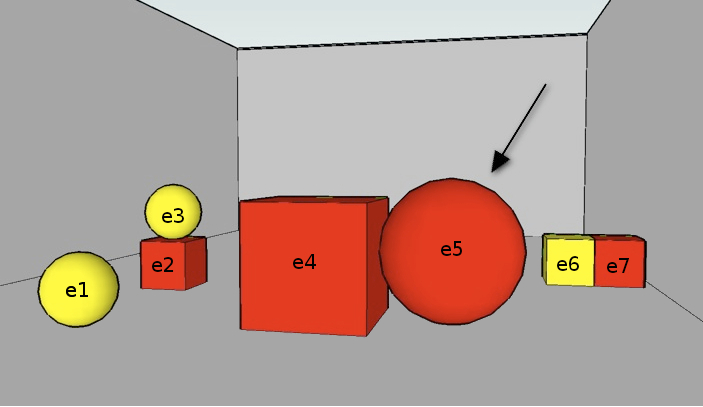
\includegraphics[width=\textwidth]{images/22.jpg}
%\vspace*{1cm}
%\caption{Input scene}
\label{GRE3D7-stimulus-22}
\end{subfigure}
%\hspace*{-0.35cm}
\begin{subfigure}{.5\textwidth}
  \centering
%\includegrahics[width=\textwidth]{images/22sinletras.jpg}
%%\caption{Ejemplo de contexto}
%\label{GRE3D7-stimulus1-b}
%\vspace*{1cm}
\begin{picture}(250,0)
\put(0,-80){\begin{tikzpicture}
  [
    n/.style={circle,draw,inner sep=1.5pt,node distance=1.5cm},
		 aArrow/.style={->, >=stealth, semithick, shorten <= 1pt, shorten >= 1pt},
  ]
 \node[n,label=below:{
    \relsize{-2}$\begin{array}{c}
		  \nLeft\\[-3pt]
      \nSmall\\[-3pt] 
      \nYellow \\[-3pt] 
      \nBall\end{array}$}] (a) {$e_1$};
 \node[n,label=below:{
    \relsize{-2}$\begin{array}{c} 
		  \nLeft\\[-3pt]
      \nSmall\\[-3pt] 
      \nRed\\[-3pt] 
      \nCube\end{array}$}, right of=a] (b) {$e_2$};
 \node[n,label=above:{
    \relsize{-2}$\begin{array}{c}
      \nTop\\[-3pt]
      \nLeft\\[-3pt]
      \nSmall\\[-3pt] 
      \nYellow\\[-3pt] 
      \nBall\end{array}$}, above of=b] (c) {$e_3$};
 \node[n,label=below:{
    \relsize{-2}$\begin{array}{c}
      \nLarge\\[-3pt] 
      \nRed\\[-3pt] 
      \nCube\end{array}$}, right of=b] (d) {$e_4$};
 \node[n,label=below:{
    \relsize{-2}$\begin{array}{c}
      \nLarge\\[-3pt] 
      \nRed\\[-3pt] 
      \nBall\end{array}$}, right of=d] (e) {$e_5$};
 \node[n,label=below:{
    \relsize{-2}$\begin{array}{c}
      \nSmall\\[-3pt] 
      \nYellow\\[-3pt] 
      \nCube\end{array}$}, right of=e] (f) {$e_6$};
 \node[n,label=below:{
    \relsize{-2}$\begin{array}{c}
      \nSmall\\[-3pt]
      \nRed\\[-3pt] 
      \nCube\end{array}$},  right of=f] (g) {$e_7$};
 \draw [aArrow,bend right=40] (b) to node[auto,swap]{\relsize{-3}$\nBelow$} (c);
 \draw [aArrow,bend right=40] (c) to node[auto,swap]{\relsize{-3}$\texttt{ontop}$} (b);
 \draw [aArrow,bend right=40] (d) to node[auto,swap]{\relsize{-3}$\nLeftof$} (e);
 \draw [aArrow,bend right=40] (e) to node[auto,swap]{\relsize{-3}$\nRightof$} (d);
 \draw [aArrow,bend right=40] (f) to node[auto,swap]{\relsize{-3}$\nLeftof$} (g);
 \draw [aArrow,bend right=40] (g) to node[auto,swap]{\relsize{-3}$\nRightof$} (f);
 %\draw[dotted] (-0.5,-1.3) rectangle (8,3.1);
 \draw[dotted] (-0.5,-1.8) rectangle (8,3.7);
 \end{tikzpicture}}
 \end{picture}
%\end{flushleft}
\end{subfigure}
\caption{Contexto y modelo del ejemplo de ejecuci\'on.}\label{fig4-9}
\end{figure}

Empezamos, estamos en la primer iteraci\'on del algoritmo. La primer relaci\'on a considerar por su R.\puse\ es \texttt{ball}. \texttt{ball}.\puse\ es mayor que \texttt{ball}.\randomuse, recordemos que la relaci\'on \texttt{ball} se a\~nadir\'a a \RE si su interpretaci\'on tiene al menos un elemento, $\interp{\top \sqcap \texttt{ball}}$\footnote{Como las relaciones unarias se transformaron en binarias, la f\'ormula que el algoritmo agregar\'a ser\'a $\top \sqcap \exists\ \texttt{ball}.\top$. Aqu\'i escribimos $\top \sqcap \texttt{ball}$ por simplicidad.} no tiene que ser vac\'io, y su interpretaci\'on tiene que ser distinta de $\interp{\top}$. Las tres condiciones se cumplen y \RE entonces es \{$\top$, \texttt{ball}\}. Se ven los elementos de $\interp{\texttt{ball}}$ enmarcados en la Figura~\ref{fig-modelo3} ($e_1$, $e_3$, $e_5$). El conjunto $\interp{\top}$ tambi\'en est\'a enmarcado e incluye todos los elementos del modelo.

\begin{figure}[H]
\begin{center}
\frame{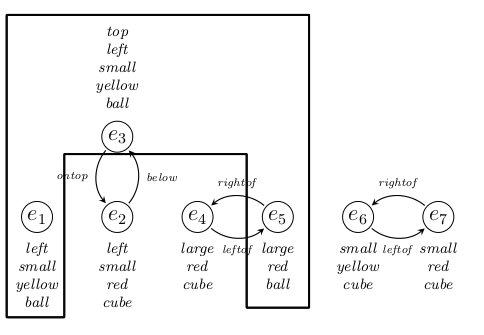
\includegraphics[width=11cm]{images/im/1ball.png}}\\[0pt]
\caption{El cuadro mayor indica elementos que satisfacen $\top$. El recuadro m\'as chico elementos que satisfacen la f\'ormula \texttt{ball}.}
\label{fig-modelo3}
\end{center}
\end{figure}

La siguiente propiedad a considerar es \texttt{cube}, tambi\'en supera la probabilidad \texttt{cube}.\randomuse). Realizando el mismo procedimiento antes mencionado, queda \RE =\{$\top$, \texttt{ball}, \texttt{cube}\} donde $\interp{\texttt{ball}}$ = $\{e_1,e_3,e_5\}$ y
$\interp{\texttt{cube}}$ = $\{e_2, e_4, e_6, e_7\}$. Notar que las particiones de  \texttt{ball} y \texttt{cube} hacen que $\top$ no agregue informaci\'on es decir $\top$ est\'a subsumida, por lo tanto podemos borrarla. Quedando las particiones como se muestran en la Figura~\ref{fig-modelo4}.

\begin{figure}[H]
\begin{center}
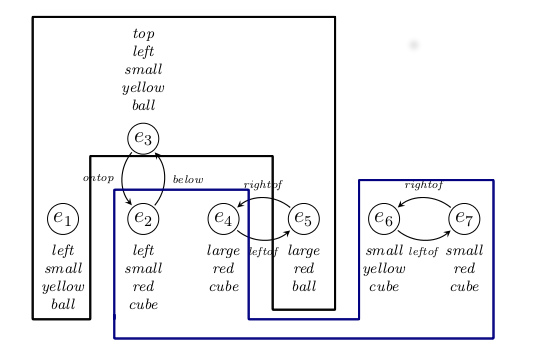
\includegraphics[width=11cm]{images/im/2ball-cube.jpg}
%\externalfigure[file][frame=on]
\caption{Conjuntos de elementos que satisfacen las f\'ormulas \texttt{ball} y \texttt{cube}.}
\label{fig-modelo4}
\end{center}
\end{figure}

La siguiente propiedad es \texttt{red}, que tambi\'en supera la probabilidad \texttt{red}.\randomuse. Tenemos que  
$\interp{\texttt{red}}$ = $\{e_2, e_4, e_5, e_7\}$, haciendo la intersecci\'on con la $\interp{.}$ de cada f\'ormula en \RE obtenemos, 
$\{e_5\}$ y $\{e_2, e_4, e_7\}$. Las interpretaciones de las f\'ormulas en \RE se pueden ver en la Figura~\ref{fig-modelo9}. El conjunto \RE hasta el momento es $\{\texttt{ball}, \texttt{cube}, \texttt{ball} \sqcap \texttt{red}, \texttt{cube} \sqcap \texttt{red}\}$. Cuando la interpretaci\'on de una f\'ormula es un conjunto singleton lo indicamos con una elipsis en lugar de un recuadro.

\begin{figure}[H]
\begin{center}
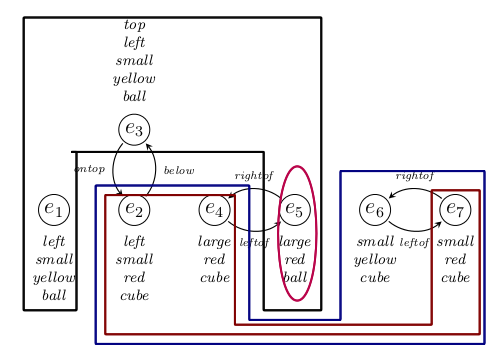
\includegraphics[width=11cm]{images/im/rojo.png}
\caption{Conjuntos de elementos que cumplen las f\'ormulas: $\texttt{ball}, \texttt{ball} \sqcap \texttt{red}, \texttt{cube},\texttt{cube} \sqcap \texttt{red}$.}
\label{fig-modelo9}
\end{center}
\end{figure}    

Ahora es el turno de \texttt{large} que tambi\'en supera la probabilidad R.\randomuse. Tenemos que $\interp{\texttt{large}}$ = $\{e_4, e_5\}$, haciendo la intersecci\'on con las dem\'as f\'ormulas que tenemos hasta el momento nos queda \RE de la siguiente manera:
 $\{\texttt{ball}, \texttt{cube}, \texttt{ball} \sqcap \texttt{red} \sqcap \texttt{large}, \texttt{cube} \sqcap \texttt{red} ,\texttt{cube} \sqcap \texttt{red} \sqcap \texttt{large} \}$. Notar que como estamos en la primera iteraci\'on, y no chequeamos informatividad, se agreg\'o \texttt{large} a $\texttt{ball} \sqcap \texttt{red}$ se agreg\'o sobreespecificando, porque no divid\'ia el conjunto. %Las particiones se muestran en la Figura \ref{fig-modelo9b}.

%\begin{figure}[h]
%\begin{center}
%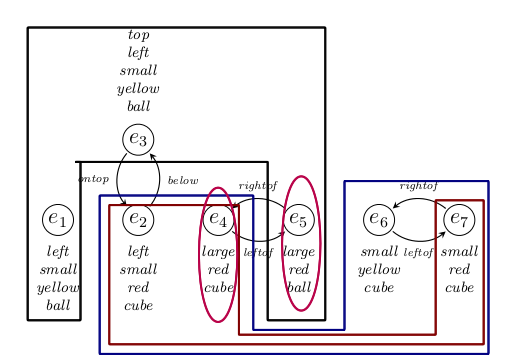
\includegraphics[width=11cm]{images/im/large.png}
%\caption{Cuadros indicando particiones de elementos que cumplen las f\'ormulas: $\texttt{ball}, \texttt{ball} \sqcap \texttt{red} \sqcap \texttt{large}, \texttt{cube},\texttt{cube} \sqcap \texttt{red}, \texttt{cube} \sqcap \texttt{red} \sqcap \texttt{large}$.}
%\label{fig-modelo9b}
%\end{center}
%\end{figure}

La siguiente relaci\'on es \texttt{ontop}, la cual supera la probabilidad \texttt{ontop}.\randomuse. $e_3$ es el \'unico elemento que est\'a \texttt{ontop} quedando \RE= $\{\texttt{ball}, \texttt{cube}, \texttt{ball} \sqcap \texttt{red} \sqcap \texttt{large}, \texttt{cube} \sqcap \texttt{red}, \texttt{cube} \sqcap \texttt{red} \sqcap \texttt{large}, \texttt{ball} \sqcap \exists \texttt{ontop}.(\texttt{cube} \sqcap \texttt{red})\}$. Los conjuntos resultantes se muestran en la Figura \ref{fig-modelo9c}.

\begin{figure}[H]
\begin{center}
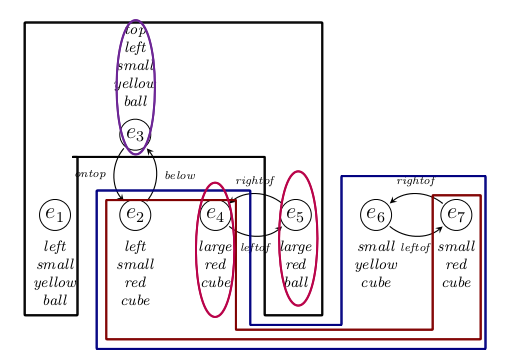
\includegraphics[width=11cm]{images/im/ontop.png}
\caption{Cuadros indicando particiones de elementos que cumplen las f\'ormulas: $\texttt{ball}, \texttt{ball} \sqcap \texttt{red} \sqcap \texttt{large}, \texttt{cube},\texttt{cube} \sqcap \texttt{red}, \texttt{cube} \sqcap \texttt{red} \sqcap \texttt{large},\texttt{ball} \sqcap \exists \texttt{ontop}. \texttt{cube} \sqcap \texttt{red}$.}
\label{fig-modelo9c}
\end{center}
\end{figure}

Siguiendo con \texttt{yellow}, tenemos que $\interp{\texttt{yellow}}$ = $\{e_1, e_3, e_6\}$ y obtenemos \RE= $\{\texttt{ball},\texttt{ball} \sqcap \texttt{yellow}, \texttt{cube}, \texttt{cube} \sqcap \texttt{yellow}, \texttt{ball} \sqcap \texttt{red} \sqcap \texttt{large}, \texttt{cube} \sqcap \texttt{red}, \texttt{cube} \sqcap \texttt{red} \sqcap \texttt{large}, \texttt{yellow} \sqcap \texttt{ball} \sqcap \exists \texttt{ontop}.\texttt{cube} \sqcap \texttt{red} \}$. Algunas relaciones se agregaron sobreespecificando, ya que todav\'ia estamos en el primer ciclo.
Aqu\'i ya borramos la f\'ormula \texttt{ball} porque estaba subsumida, y la f\'ormula \texttt{cube} tambi\'en. Se muestran las particiones resultantes en la Figura~\ref{fig-modelo9d}, luego de haber borrado las f\'ormulas subsumidas.

\begin{figure}[H]
\begin{center}
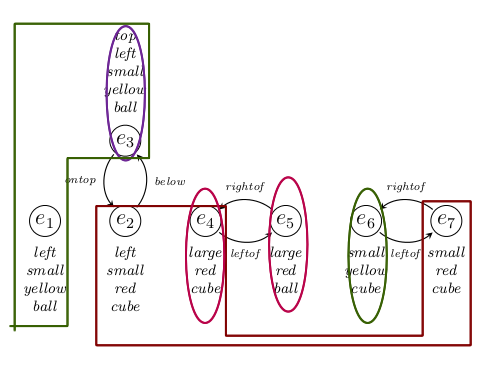
\includegraphics[width=11cm]{images/im/yellow.png}

\caption{Cuadros indicando particiones de elementos que cumplen las
  f\'ormulas: 
$\texttt{ball} \sqcap \texttt{red} \sqcap \texttt{large}$,
$\texttt{cube} \sqcap \texttt{red}$, 
$\texttt{cube} \sqcap \texttt{red} \sqcap \texttt{large}$,
$\texttt{ball} \sqcap \exists \texttt{ontop}. \texttt{cube} \sqcap
\texttt{red}$, 
$\texttt{cube} \sqcap \texttt{yellow}$, 
$\texttt{ball} \sqcap \texttt{yellow}$.}
\label{fig-modelo9d}
\end{center}
\end{figure}


Las dem\'as propiedades no pasan la probabilidad R.\randomuse, por lo tanto salimos del primer ciclo, e incrementamos las probabilidades con R.\incuse, hasta que alguna relaci\'on R es tal que R.\randomuse <= R.\puse, quedando como se muestran en la Tabla \ref{prob-inc2}.

%Las dem\'as propiedades y no pasaron la probabilidad random del algoritmo, pero a\'un tenemos particiones con m\'as de un elemento, y las probabilidades de uso son menores que 1, por lo tanto se aumentan las probabilidades de uso en 0.2 (siendo ) para cada propiedad quedando:


%\begin{table}[h]
%\begin{center}
%\footnotesize{
%\begin{tabular} {  l c c c c c c c c c c c }
%\hline
%%\multicolumn{1}{c}{}
%%&\multicolumn{1}{c}{Domain}
%%&\multicolumn{3}{c}{Descriptions}\\

%R				&{\it ball}			& {\it cube}	& {\it red}	  & {\it large} & {\it ontop} & {\it yellow} & {\it small} & {\it rightof} & {\it leftof}   & {\it top}& {\it left}   \\
%\hline
%R.\puse	& 1.0			& 1.0		& 0.9824	& 0.4056 & 0.3424 & 0.32   & 0.2856 & 0.2056& 0.2 &0.2 &0.2  \\ \hline
%R.\randomuse & 0.3234 & 0.5607 &0.8771 &0.1256 &0.1424 &0.0398 &0.7099 &0.2184 &0.8570 &0.8166 &0.2026\\ \hline
%R.\incuse & 0&0&0.0044& 0.1486& 0.1644& 0.17& 0.1786& 0.1986& 0.2 & 0.2 & 0.2\\ \hline

%\end{tabular}
%}
%\end{center}
%\vspace*{-.5cm} 
%\caption{Probabilidad R.\puse\ de las propiedades y relaciones, incrementadas en R.\incuse luego del primer ciclo de ejecuci\'on.}\label{prob-inc1}
%\vspace*{1cm}
%\end{table}

Las interpretaciones de las f\'ormulas hasta el momento e ilustradas gr\'aficamente en la Figura \ref{fig-modelo9d} son:

\begin{tabular}{l}
$\interp{ \texttt{ball}} = \{e_1, e_3, e_5\}$ \\
$\interp {\texttt{ball} \sqcap \texttt{yellow}} = \{e_1, e_3\}$\\
$\interp {\texttt{cube} \sqcap \texttt{yellow} }= \{e_6\}$ \\
$\interp {\texttt{ball} \sqcap \texttt{red} \sqcap \texttt{large}} = \{e_5\}$ \\
$\interp {\texttt{cube} \sqcap \texttt{red} }= \{e_2, e_4, e_7\}$ \\
$\interp {\texttt{cube} \sqcap \texttt{red} \sqcap \texttt{large}} = \{e_4\}$  \\
$\interp {\texttt{yellow} \sqcap \texttt{ball} \sqcap \exists \texttt{ontop}.\texttt{cube}} = \{e_3\} $
\end{tabular}



De ahora hasta que termine el algoritmo, no se agregar\'an propiedades por sobreespecificaci\'on. Notar que ya tenemos 4 conjuntos singleton, los cuales no cambiar\'an hasta el final de la ejecuci\'on. El algoritmo contin\'ua porque siguen quedando clases para refinar, las cuales son $\texttt{ball} \sqcap \texttt{yellow}$ y $\texttt{cube} \sqcap \texttt{red}$.

\begin{table}[h]
\begin{center}
\footnotesize{
\begin{tabular} {  l c c c c c c c c c c c c}
\hline
%\multicolumn{1}{c}{}
%&\multicolumn{1}{c}{Domain}
%&\multicolumn{3}{c}{Descriptions}\\

R				&{\it ball}			& {\it cube}	& {\it red}	  & {\it large} & {\it ontop} & {\it yellow} & {\it small} & {\it rightof} & {\it leftof}   & {\it top}& {\it left}& {\it below}   \\
\hline
R.\puse	& 1.0			& 1.0		& 0.9868	& 0.5542 & 0.5068 & 0.49   & 0.4642 & 0.4042& 0.4 &0.4 &0.4  &0.4\\ \hline
R.\randomuse & 0.323 & 0.560 &0.877 &0.125 &0.142 &0.039 &0.709 &0.218 &0.857 &0.816 &0.202 &0.13\\ \hline
R.\incuse & 0&0&0.004& 0.148& 0.164& 0.17& 0.178& 0.198& 0.2 & 0.2 & 0.2 &0.2\\ \hline

\end{tabular}
}
\end{center}
\vspace*{-.5cm} 
\caption{Probabilidad R.\puse\ de las propiedades y relaciones, incrementadas en R.\incuse luego del primer ciclo de ejecuci\'on.}\label{prob-inc2}
\vspace*{1cm}
\end{table}

La relaci\'on \texttt{small} no pasa la probabilidad random, pero \texttt{rightof} s\'i. Continuamos con \texttt{rightof}. Agregamos $\texttt{cube} \sqcap \texttt{red} \sqcap \exists \texttt{rightof}. \texttt{cube} \sqcap \texttt{yellow}$.
%, quedando las particiones como se muestra en la Figura \ref{fig-modelo9e}.

%\begin{figure}[ht]
%\begin{center}
%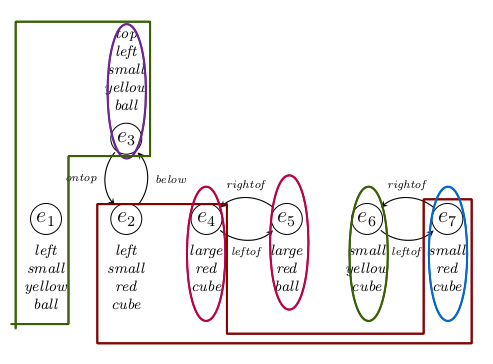
\includegraphics[width=11cm]{images/im/rightof.png}
%\caption{Cuadros indicando particiones de elementos que cumplen las f\'ormulas: $\texttt{ball} \sqcap \texttt{red} \sqcap \texttt{large},\texttt{cube} \sqcap \texttt{red}, \texttt{cube} \sqcap \texttt{red} \sqcap \texttt{large},\texttt{ball} \sqcap \exists \texttt{ontop}. \texttt{cube} \sqcap \texttt{red}, \texttt{cube} \sqcap \texttt{yellow}, \texttt{ball} \sqcap \texttt{yellow}, \texttt{cube} \sqcap \texttt{red} \sqcap \exists \nRightof. \texttt{cube} \sqcap \texttt{yellow}$.}
%\label{fig-modelo9e}
%\end{center}
%\end{figure}

La siguiente que pasa la probabilidad random es \texttt{left}. Se agrega la f\'ormula $\texttt{left} \sqcap \texttt{red} \sqcap \texttt{cube}$, y su correspondiente interpretaci\'on. Se muestran los conjuntos resultantes en la Figura \ref{fig-modelo9f}. $\texttt{cube} \sqcap \texttt{red}$ se elimina porque es redundante.

\begin{figure}[H]
\begin{center}
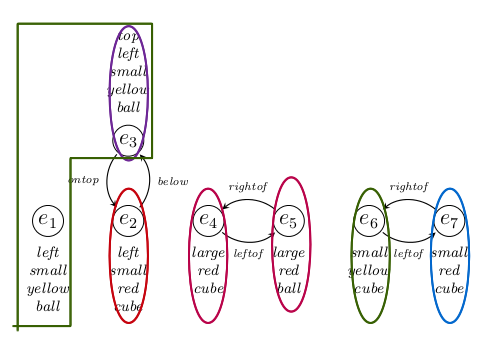
\includegraphics[width=11cm]{images/im/left.png}
\caption{Cuadros indicando particiones de elementos que cumplen las f\'ormulas: $\texttt{ball} \sqcap \texttt{red} \sqcap \texttt{large}, \texttt{cube} \sqcap \texttt{red} \sqcap \texttt{large},\texttt{ball} \sqcap \exists \texttt{ontop}. \texttt{cube} \sqcap \texttt{red}, \texttt{cube} \sqcap \texttt{yellow}, \texttt{ball} \sqcap \texttt{yellow}, \texttt{cube} \sqcap \texttt{red} \sqcap \exists \texttt{rightof}. \texttt{cube} \sqcap \texttt{yellow}$, $\texttt{left} \sqcap \texttt{red} \sqcap \texttt{cube}$.}
\label{fig-modelo9f}
\end{center}
\end{figure}

\texttt{small} no se agrega a $\texttt{ball} \sqcap \texttt{yellow}$ porque no es informativo. 
Subiendo un par de veces las probabilidades de uso, el algoritmo finaliza por no poder hacer m\'as refinamientos quedando las siguientes clases y sus interpretaciones:

\begin{tabular}{l}
$\interp{\texttt{ball} \sqcap \texttt{yellow}} = \{e_1, e_3\}$  \\
$\interp{\texttt{cube} \sqcap \texttt{yellow} }= \{e_6\}$ \\
$\interp{\texttt{ball} \sqcap \texttt{red} \sqcap \texttt{large}} = \{e_5\}$ \\
%$\interp{\texttt{cube} \sqcap \texttt{red}} = \{e_2, e_4, e_7\}$ \\
$\interp{\texttt{left} \sqcap \texttt{cube} \sqcap \texttt{red}} = \{e_2\}$ \\
$\interp{\texttt{cube} \sqcap \texttt{red} \sqcap \texttt{large}} = \{e_4\}$  \\
$\interp{\texttt{yellow} \sqcap \texttt{ball} \sqcap \exists \texttt{ontop}.\texttt{cube} \sqcap \texttt{red}} = \{e_3\}$ \\ 
$\interp{\texttt{cube} \sqcap \texttt{red} \sqcap \exists \texttt{rightof}. \texttt{cube} \sqcap \texttt{yellow}} = \{e_7\}$
\end{tabular}

Conclu\'imos que el lenguaje elegido $\el$ no pueden identificar a $e_1$ en el modelo. Si us\'aramos $\alc$, que contiene negaci\'on $e_1$ se podr\'ia distinguir de $e_3$. Los dem\'as elementos s\'i quedan en clases singleton y son expresiones referenciales podr\'ian realizarse como sigue:
{\it el cubo amarillo} es $e_6$, {\it la bola grande roja} es $e_5$, {\it el cubo rojo grande} es $e_4$, {\it el cubo rojo que est\'a a la derecha del cubo amarillo} es $e_7$, $e_3$ es {\it la bola amarilla sobre el cubo rojo} y $e_2$ es {\it el cubo rojo de la izquierda}.
 
%Otra vez las probabilidades random superan a las de la lista, recalculamos las probabilidades sumando R.\incuse a cada \puse, quedando como muestra la Tabla \ref{probabilidades-ejemplo-ejecucion3}.

%\begin{table}[h]
%\begin{center}
%\footnotesize{
%\begin{tabular} {  l c c c c c c c c c }
%\hline
%%\multicolumn{1}{c}{}
%%&\multicolumn{1}{c}{Domain}
%%&\multicolumn{3}{c}{Descriptions}\\

%R				&{\it ball}			& {\it cube}	& {\it red}	  & {\it large} & {\it ontop} & {\it yellow} & {\it small} & {\it rightof} & {\it leftof}   \\
%\hline
%R.\puse	& 1.0			& 1.0		& 0.9868	& 0.5542 & 0.5068 & 0.49   & 0.4642 & 0.4042& 0.4 \\
%\hline

%\end{tabular}
%}
%\end{center}
%\vspace*{-.5cm} 
%\caption{Probabilidad de las propiedades y relaciones de la figura de ejemplo, incrementadas en R.\incuse.}\label{probabilidades-ejemplo-ejecucion3}
%\vspace*{1cm}
%\end{table}



\subsection{Asegurando terminaci\'on generando expresiones relacionales}

Uno de los problemas que ten\'ian otros algoritmos es que no siempre terminaban como explicamos en el Cap\'itulo \ref{sec:seleccion}. Para asegurar terminaci\'on nosotros incrementamos las probabilidades aleatorias en cada ciclo, hasta que alcancen 1. Definimos MaxIterations como la cantidad m\'axima de iteraciones que vamos a permitir, y calculamos R.\incuse es cuanto vamos a incrementar la probabilidad de R en cada ciclo, R.\incuse = (1 -R.\puse) / MaxIterations, con esto nos aseguramos que en MaxIterations todas lleguen a 1, y en consecuencia el algoritmo termine, ya que en el c\'odigo, se incrementa R.\puse con R.\incuse y sale del ciclo principal si para todas las R, R.\puse son mayores o iguales a 1.

El fragmento del Algoritmo \ref{algo:bisim-l} definido por el while es un algoritmo de punto fijo, se refinan las particiones hasta que en alg\'un momento no se pueden hacer m\'as refinamientos, se dice que el algoritmo llego a un punto fijo, en el que no le es posible progresar. \RE se mantiene sin modificaciones. Los conjuntos se van haciendo m\'as chicos en las sucesivas iteraciones y considerando que la cantidad de elementos del modelo y las relaciones son finitas, se llega al punto fijo en una cantidad finita de pasos y el algoritmo siempre termina.

Nuestro algoritmo permite generar relaciones binarias con otros objetos e incluir descripciones de los dem\'as objetos (en las ERs). No tiene preferencia por las relaciones ni por las propiedades proposicionales (como otros algoritmos descriptos de trabajo previo), en el sentido de que va a incluirlas de acuerdo a la probabilidad de uso que ellas tengan, las cuales fueron calculadas o aprendidas de un corpus. En el ejemplo de ejecuci\'on anterior mostramos que el algoritmo agreg\'o la f\'ormula $\texttt{cube} \sqcap \texttt{red} \sqcap \exists \texttt{rightof}. \texttt{cube} \sqcap \texttt{yellow}$ que incluye la relaci\'on binaria \texttt{rightof}.

\subsection{Generando no-determin\'isticamente sobreespecificaci\'on}

Al iniciar el algoritmo calcula para cada R, R.\randomuse que es un n\'umero aleatorio entre 0 y 1, ese n\'umero va a hacer que el algoritmo sea no-determin\'istico, ya que, el algoritmo usar\'a R para refinar las clases solamente si 
R.\randomuse >= R.\puse. Por lo tanto y considerando que en las siguientes ejecuciones R.\randomuse ser\'an distintos, va a poder generar distintas ERs.

El algoritmo hace caso omiso de la restricci\'on de informatividad (es decir, que permite la inclusi\'on de nuevas relaciones
en la descripci\'on, incluso si no refinan la clase asociada) \emph{pero s\'olo durante el
primer ciclo del algoritmo}. Es decir, durante el primer ciclo del repeat principal del algoritmo, se permitir\'a la inclusi\'on de todas las relaciones que no trivializan la
descripci\'on (es decir, la clase asociada no est\'a vac\'{i}a y que no son redundantes). Debido a que esto se hace s\'olo durante
el primer ciclo, sabemos que no aparecer\'an propiedades repetidas en las ERs generadas (como \texttt{green green ball}).
En los ciclos restantes, se a\~nadir\'an propiedades adicionales s\'olo si son de car\'acter informativo.
Este dise\~no del algoritmo que permite sobreespecificaci\'on est\'a inspirado en la obra de \cite{keysar:Curr98} sobre el egocentrismo y la producci\'on del lenguaje natural. Keysar et al. argumentan que cuando se produce el lenguaje, el hablante no identifica un\'ivocamente al target desde el principio, sino que  
es m\'as bien un ajuste de \'ultimo momento. Los hablantes producen ERs primero egoc\'entricamente, agregando aquellas propiedades m\'as prominentes por m\'as de que no sean informativas. Pero luego las ajustan de modo que el destinatario de la ER sea capaz de identificarla un\'ivocamente. El primer paso, egoc\'entrico, es un proceso
heur\'istico basado en un modelo de la prominencia de la propiedades de la escena que contiene el target. Nuestra definici\'on de
\puse\ est\'a destinada a capturar las prominencias de las propiedades de diferentes escenas y targets. Los valores de \puse\
cambian en relaci\'on a la escena considerada. Esto est\'a en contraste con el trabajo previo en GER descripto en el Cap\'itulo \ref{sec:seleccion} donde
la prominencia de una propiedad es constante en un dominio. Keysar et al. argumentan que la raz\'on del procedimiento de 
generar-y-ajustar puede tener que ver con las limitaciones de procesamiento de informaci\'on de la
mente: si la heur\'istica que gu\'ia la fase egoc\'entrica est\'a bien sintonizada, consigue una adecuada ER al principio
y rara vez requerir\'a ajustes. Se observa un comportamiento similar
con nuestro algoritmo: cuando los valores de \puse\ son
aprendidos del dominio, el algoritmo no es
s\'olo es m\'as preciso, sino que tambi\'en es mucho m\'as r\'apido que cuando se utilizan valores de \puse\ aleatorios.  


%\subsection{Generando ER para plurales}
%
%Este algoritmo devuelve ER para todos los elementos del contexto, 
%esto implica que podr\'iamos dar expressiones referenciales de un conjunto de elementos.
%
%Por ejemplo queremos identificar a $e_1$ y $e_5$ 
%siendo resultados dados por el algoritmo que $e_1$
%ball, yellow, small
%y $e_5$ ball, red
%
\subsection{Generando expresiones plurales}
\label{sec:genera_plural}
Como dijimos el algoritmo puede dar ERs para todos los elementos del modelo. Pero tambi\'en le agregamos al input un target, que puede ser singleton o un conjunto de elementos del modelo.

Para dar las ERs plurales simplemente damos la conjunci\'on de las ERs de los elementos que pertenezcan al conjunto target. El algoritmo en algunas ocasiones particiona por alguna relaci\'on en la que quedan los elementos del target juntos, generando as\'i expresiones referenciales colectivas, pero esto no pasa normalmente. 

En la Secci\'on \ref{sec:plural} se muestra un caso de estudio de ER plurales.

\section{Notas finales y linkeo del cap\'itulo}
\label{sec:link-algoritmo}

En este cap\'itulo se explic\'o la entrada y salida de un algoritmo probabil\'istico. Una de las entradas es el modelo, el cual es una representaci\'on de la figura considerada. Otra es una distribuci\'on de probabilidades finita, la cual explicamos como obtenerla en 2 casos. Primero en el caso que hay corpus disponible para la escena considerada y en casos donde al no haber corpus disponible proponemos una aproximaci\'on usando aprendizaje autom\'atico. Se explic\'o el algoritmo en detalle y se ilustr\'o con un ejemplo de ejecuci\'on. Se explic\'o c\'omo hace el algoritmo para conseguir las siguientes caracter\'isticas: asegurar terminaci\'on, generar ER relacionales, generar ER no-determin\'isticas y generar sobreespecificaci\'on.
El dise\~no del algoritmo est\'a inspirado en el modelo cognitivo de generaci\'on de expresiones referenciales de \cite{keysar:Curr98}. En el Cap\'itulo \ref{sec:evaluacion} veremos que este algoritmo es capaz de generar rankings de ERs cercanos a los encontrados en corpora.
El algoritmo presentado en este cap\'itulo introduce una familia de algoritmos que extiende probabil\'isticamente a los algoritmos presentados en el Cap\'itulo \ref{sec:intro_logica}. Se explicaron los detalles de la subrutina \textit{add} para el lenguaje \EL. Las definiciones de \textit{add} para otros lenguajes como \ALC o \EPFOL son similares.
Como se discuti\'o en el Cap\'itulo \ref{sec:intro}, los dominios realistas de posibles aplicaciones de la GER contienen incertidumbre. En este cap\'itulo modelamos esa incertidumbre como las probabilidades de usar una caracter\'istica en una ER. 
Los algoritmos presentados en este cap\'itulo pueden tambi\'en ser usados con probabilidades provenientes de confidence scores de sensores, por ejemplo, para modelar otros tipos de incertidumbre.
En el Cap\'itulo \ref{sec:corpus} evaluamos estos algoritmos sobre un corpus de descripciones de mapas, el corpus ZOOM.
% generar ER para plurales.
%
%En el c\'alculo de probabilidades de uso de las palabras con nuestra versi\'on simplista, podemos ver cosas interesantes como por ejemplo que {\it ball} tiene una \puse\ alta, ya que en el corpus considerado todos los targets son {\it ball}, en cambio la probabilidad de {\it cube} no es tan alta y depende de la discernibilidad, si aparece, aparece en la descripci\'on del landmark. Para {\it blue} y {\it green} el valor de \puse\ depende de si el target es {\it blue} o {\it green}, entonces si el target es {\it blue}, le da un valor alto a {\it blue} y bajo a {\it green} y viceversa. Las relaciones {\it ontop}, {\it leftof} y {\it rightof} dependen fuertemente si el target tiene o no esa relaci\'on y en caso de tenerla igualmente la \puse\ no es muy alta, esto indica que en un porcentaje del 30\% por ejemplo se usa {\it ontop} y en menos del 3\% {\it leftof} o {\it rightof}, ya reportado en trabajo previo. Vimos que el tama\~no es m\'as frecuente usado para sobreespecificaci\'on cuando el target y el landmark tienen el mismo tama\~no (es usado en ERs sobreespecificadas el 49\% cuando el target y el landmark comparten el tama\~no, y s\'olo el 25\% cuando no lo comparten).
%Hay algunas relaciones complejas entre las caracter\'{i}sticas de las escenas que no somos capaces de
%capturar. La caracter\'{i}stica m\'as importante del dominio \textit{GRE3D7}
%que no somos capaces de aprender, y tiene un impacto en nuestro desempe\~no, es que
%las propiedades de tama\~no (es decir, small y large) se utilizan mucho
%m\'as cuando el target no puede ser identificado s\'olo con las propiedades taxon\'omicas absolutas 
%(verde y azul) y (ball y cube). En otras palabras, en el corpus \textit{GRE3D7} se utiliza el tama\~no con m\'as frecuencia (90,2 \%)
%cuando la ER resultante no es sobreespecificada y cuando si es sobreespecificada el (34 \%). \\

